The given equation \eqref{eq:solutions/13/5/eq:0} can be written as
\begin{align}
\vec{x}^T\myvec{1 & 3 \\ 3 & 9}\vec{x} +2\myvec{2 &6}\vec{x}-5=0\label{eq:solutions/13/5/eq:1}\\
\vec{V} = \myvec{1 & 3 \\ 3 & 9} \quad \vec{u} = \myvec{2 \\ 6} \quad f= -5 \label{eq:solutions/13/5/eq:2}
\end{align}
Equation \eqref{eq:solutions/13/5/eq:0} represents pair of straight line as,
\begin{align}
D = \mydet{1&3&2\\3&9&6\\2&6&-5} = 0
\end{align}
Vector form of straight lines,
\begin{align}
\vec{n_1}^T\vec{x}= \vec{c_1}\\
\vec{n_2}^T\vec{x} = \vec{c_2}
\end{align}
Equating their product with \eqref{eq:solutions/13/5/eq:1}
\begin{align}
(\vec{n_1}^T\vec{x} -\vec{c_1})(\vec{n_2}^T\vec{x} - \vec{c_2})= \vec{x}^T\myvec{1 & 3 \\ 3 & 9}\vec{x} +2\myvec{2 &6}\vec{x}-5
\end{align}
\begin{align}
\vec{n_1}*\vec{n_2}=\myvec{1\\6\\9}\label{eq:solutions/13/5/eq:3}\\
c_2\vec{n_1}+c_1\vec{n_2} = -2\myvec{2\\6}\\
c_1c_2 = -5
\end{align}
The slopes of the lines can be given by roots of the equation,
\begin{align} 
cm^2+2bm+a=0 \label{eq:solutions/13/5/eq:4}\\
m_i = \frac{-b\pm \sqrt{-\mydet{\vec{V}}}}{c}\label{eq:solutions/13/5/eq:5}\\
\vec{n_i}=k_i\myvec{-m_i\\1}\label{eq:solutions/13/5/eq:6}
\end{align}
From \eqref{eq:solutions/13/5/eq:1} equation \eqref{eq:solutions/13/5/eq:4} becomes
\begin{align}
9m^2+6m+1=0
\end{align}
Using \eqref{eq:solutions/13/5/eq:2},
\begin{align}
\mydet{\vec{V}} = \mydet{1 & 3\\ 3 & 9} = 0
\end{align}
Substituting the values in \eqref{eq:solutions/13/5/eq:5},
\begin{align}
m_i = \frac{-3\pm 0}{9}\\
m_1= m_2 = \frac{-1}{3} \label{eq:solutions/13/5/eq:7}
\end{align}
Substituting values in \eqref{eq:solutions/13/5/eq:6}
\begin{align}
\vec{n_1}=k_1\myvec{\frac{1}{3}\\1}\\
\vec{n_2}=k_2\myvec{\frac{1}{3}\\1}
\end{align}
Using the above values in \eqref{eq:solutions/13/5/eq:3},
\begin{align}
k_1k_2 = 9
\end{align}
Taking $k_1=3$ and $k_2 = 3$ we get
\begin{align}
\vec{n_1}=\myvec{1\\3}\\
\vec{n_2}=\myvec{1\\3}
\end{align}
Verifying $\vec{n_1}$ and $\vec{n_2}$ by computing the convolution by representing $\vec{n_1}$ as Toeplitz matrix,
\begin{align}
\vec{n_1}*\vec{n_2}=\myvec{1&0\\3&1\\0&3}\myvec{1\\3}=\myvec{1\\6\\9}
\end{align}
Finding the Angle between the lines,
\begin{align}
\theta = \cos^{-1}\brak{\frac{\vec{n_1}^T\vec{n_2}}{\norm{\vec{n_1}}\norm{\vec{n_2}}}}\label{eq:solutions/13/5/eq:8}\\
\vec{n_1}^T\vec{n_2} = \myvec{1&3}\myvec{1\\3} = 10 \label{eq:solutions/13/5/eq:9}\\
\norm{\vec{n_1}} = \sqrt{10}\quad \norm{\vec{n_2}}=\sqrt{10} \label{eq:solutions/13/5/eq:10}
\end{align}
Substituting \eqref{eq:solutions/13/5/eq:9} and \eqref{eq:solutions/13/5/eq:10} in \eqref{eq:solutions/13/5/eq:8} we get,
\begin{align}
\theta = \cos^{-1}(1)\\
\theta = 0^{\circ}\label{eq:solutions/13/5/eq:11}
\end{align}
From \eqref{eq:solutions/13/5/eq:7} and \eqref{eq:solutions/13/5/eq:11} shows the given equation \eqref{eq:solutions/13/5/eq:0} represents two parallel lines. Hence proved.
\begin{figure}[!ht]
\centering
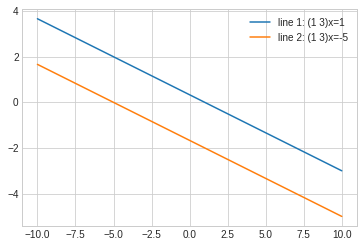
\includegraphics[width=\columnwidth]{./solutions/13/5/Straight_lines.png}
\caption{Pair of straight lines plot generated using python}
\label{eq:solutions/13/5/fig:plot}
\end{figure}
